% Gabarit pandoc des corrigés publiés (brut et guidé). Contenu sans marque ni nom de site.
% Compilation : lualatex (latexmk -lualatex).
% Le Markdown reste la source unique : ne pas éditer ce fichier .tex à la main.
\documentclass[11pt,a4paper]{article}

% --- Moteur, polices (Latin Modern) et langue ---------------------------------
\usepackage{iftex}
\ifLuaTeX\else\errmessage{Ce document se compile avec lualatex}\fi
\usepackage{amsmath,amssymb,mathtools}
\usepackage{fontspec}
% mathrm=sym : \mathrm prend ses glyphes dans la police mathématique (ℓ, μ, Ω), comme KaTeX.
\usepackage[math-style=TeX,bold-style=TeX,mathrm=sym]{unicode-math}
% Repli pour les glyphes absents de Latin Modern (indices et exposants Unicode,
% flèches, filets des schémas en texte, symboles) : DejaVu, puis Latin Modern Math
% (ℓ, lettres mathématiques Unicode des légendes).
\directlua{
  luaotfload.add_fallback("repliTexte", {"DejaVuSerif:mode=harf;", "DejaVuSans:mode=harf;", "file:latinmodern-math.otf:mode=harf;"})
  luaotfload.add_fallback("repliMono", {"DejaVuSansMono:mode=harf;", "DejaVuSans:mode=harf;", "file:latinmodern-math.otf:mode=harf;"})
}
\setmainfont{Latin Modern Roman}[RawFeature={fallback=repliTexte}]
\setsansfont{Latin Modern Sans}[RawFeature={fallback=repliTexte}]
\setmonofont{Latin Modern Mono}[RawFeature={fallback=repliMono}]
\setmathfont{Latin Modern Math}
\usepackage[french]{babel}
\frenchsetup{SmallCapsFigTabCaptions=false}

% --- Mise en page --------------------------------------------------------------
\usepackage[a4paper,margin=2.2cm,headheight=14pt,footskip=1.2cm]{geometry}
\usepackage{microtype}
\setlength{\emergencystretch}{4em}
\tolerance=1500
\setlength{\parindent}{0pt}
\setlength{\parskip}{0.55\baselineskip plus 2pt minus 1pt}
\usepackage{xcolor}
% Gris nommés : babel-french rend « ! » actif dans le document.
\definecolor{gris2}{gray}{0.98}
\definecolor{gris3}{gray}{0.97}
\definecolor{gris5}{gray}{0.95}
\definecolor{gris35}{gray}{0.65}
\definecolor{gris40}{gray}{0.60}
\definecolor{gris45}{gray}{0.55}
\definecolor{gris50}{gray}{0.50}
\definecolor{gris55}{gray}{0.45}
\definecolor{gris60}{gray}{0.40}
\definecolor{gris65}{gray}{0.35}
\definecolor{gris70}{gray}{0.30}
\definecolor{gris80}{gray}{0.20}
\definecolor{gris85}{gray}{0.15}
\usepackage{graphicx}
\usepackage{float}
\usepackage{caption}
\captionsetup{font=small,labelformat=empty,justification=centering}
\usepackage{booktabs,longtable,array,multirow,calc}
\usepackage{siunitx}
\sisetup{locale=FR}
\usepackage[version=4]{mhchem}
\usepackage{listings}
\usepackage{fancyhdr}
\usepackage{lastpage}
\usepackage[most]{tcolorbox}
\usepackage{enumitem}
\setlist{nosep,leftmargin=*,topsep=2pt}
\usepackage[hidelinks,unicode]{hyperref}
\usepackage{bookmark}
\hypersetup{pdftitle={CCINP MP — Informatique 2026},pdfauthor={Rédigé par IA},pdfcreator={LaTeX},pdfsubject={Corrigé brut}}
\usepackage{xurl}

% --- Pandoc : listes, tableaux, figures ----------------------------------------
\providecommand{\passthrough}[1]{#1}
\providecommand{\tightlist}{\setlength{\itemsep}{0pt}\setlength{\parskip}{0pt}}

\makeatletter
\def\maxwidth{\ifdim\Gin@nat@width>\linewidth\linewidth\else\Gin@nat@width\fi}
\def\maxheight{\ifdim\Gin@nat@height>0.55\textheight 0.55\textheight\else\Gin@nat@height\fi}
\makeatother
\setkeys{Gin}{width=\maxwidth,height=\maxheight,keepaspectratio}
\setcounter{secnumdepth}{-\maxdimen}
\providecommand{\pandocbounded}[1]{#1}
\usepackage{longtable,booktabs,array}

% --- Code (listings) -----------------------------------------------------------
\lstset{
  basicstyle=\ttfamily\small,
  columns=fullflexible,
  keepspaces=true,
  breaklines=true,
  breakatwhitespace=false,
  postbreak=\mbox{\textcolor{gris50}{$\hookrightarrow$}\space},
  frame=single,
  rulecolor=\color{gris35},
  framesep=4pt,
  xleftmargin=5pt,xrightmargin=5pt,
  backgroundcolor=\color{gris3},
  keywordstyle=\bfseries,
  commentstyle=\color{gris65},
  stringstyle=\color{gris80},
  showstringspaces=false,
  tabsize=4,
  extendedchars=true,
  aboveskip=6pt,belowskip=6pt,
}

% --- Macros des corrigés (KaTeX ↔ LaTeX) ---------------------------------------
% Les corrigés sont écrits pour KaTeX : on définit ici ce que KaTeX connaît et
% que LaTeX n'a pas, sans jamais retoucher le Markdown.
\providecommand{\R}{\mathbb{R}}
\providecommand{\N}{\mathbb{N}}
\providecommand{\Z}{\mathbb{Z}}
\providecommand{\Q}{\mathbb{Q}}
\providecommand{\C}{\mathbb{C}}
\providecommand{\dd}{\mathrm{d}}
\providecommand{\llbracket}{\lBrack}
\providecommand{\rrbracket}{\rBrack}
\providecommand{\lBrace}{\lbrace}
\providecommand{\rBrace}{\rbrace}
\providecommand{\Box}{\square}
\providecommand{\Diamond}{\lozenge}
\providecommand{\varnothing}{\emptyset}
\providecommand{\argmax}{\operatorname*{arg\,max}}
\providecommand{\argmin}{\operatorname*{arg\,min}}
\renewcommand{\leq}{\leqslant}
\renewcommand{\geq}{\geqslant}

% Équation hors texte : réduite à la largeur de la ligne si elle déborde.
\newsavebox{\boiteequation}
\newcommand{\equationajustee}[1]{%
  \sbox{\boiteequation}{$\displaystyle #1$}%
  \ifdim\wd\boiteequation>\linewidth
    \[\resizebox{\linewidth}{!}{\usebox{\boiteequation}}\]%
  \else
    \[#1\]%
  \fi}

% --- Encadrés pédagogiques (sobres, lisibles en noir et blanc) -----------------
\tcbset{
  encadre/.style={
    enhanced,breakable,sharp corners,
    colback=white,colframe=gris55,
    boxrule=0.4pt,leftrule=2.2pt,
    left=6pt,right=6pt,top=3pt,bottom=3pt,
    before skip=6pt,after skip=6pt,
    fonttitle=\bfseries\small,coltitle=black,
    attach title to upper,after title={\quad},
    parbox=false,
  }
}
\newtcolorbox{indication}[1]{encadre,colframe=gris45,colback=gris2,title={Indication~#1}}
\newtcolorbox{methode}{encadre,colframe=gris70,title={Méthode}}
\newtcolorbox{piege}{encadre,colframe=gris85,boxrule=0.8pt,leftrule=2.2pt,title={Piège}}
\newtcolorbox{jury}{encadre,colframe=gris60,colback=gris5,title={Jury}}
\newtcolorbox{encadrenote}{encadre,colframe=gris40}

% --- Titres de section ---------------------------------------------------------
\usepackage{titlesec}
\titleformat{\section}{\Large\bfseries}{}{0pt}{}
\titleformat{\subsection}{\large\bfseries}{}{0pt}{}
\titleformat{\subsubsection}{\normalsize\bfseries}{}{0pt}{}
\titlespacing*{\section}{0pt}{14pt plus 4pt minus 2pt}{6pt}
\titlespacing*{\subsection}{0pt}{10pt plus 3pt minus 2pt}{4pt}
\titlespacing*{\subsubsection}{0pt}{8pt plus 2pt minus 2pt}{2pt}

% --- En-tête et pied de page ---------------------------------------------------
\pagestyle{fancy}
\fancyhf{}
\fancyhead[L]{\small\textsc{Corrigé brut} · CCINP MP}
\fancyhead[R]{\small Informatique 2026}
\fancyfoot[L]{\footnotesize Corrigé rédigé par IA, non officiel}
\fancyfoot[R]{\footnotesize \thepage\,/\,\pageref*{LastPage}}
\renewcommand{\headrulewidth}{0.4pt}
\renewcommand{\footrulewidth}{0pt}
\fancypagestyle{plain}{\fancyhf{}\fancyfoot[R]{\footnotesize \thepage\,/\,\pageref*{LastPage}}\fancyfoot[L]{\footnotesize Corrigé rédigé par IA, non officiel}\renewcommand{\headrulewidth}{0pt}}

\begin{document}
\thispagestyle{plain}
\begin{center}
  {\small\scshape Corrigé brut}\par\smallskip
  {\LARGE\bfseries CCINP MP — Informatique 2026\par}\medskip
  {\large CCINP · MP · Informatique · 2026\par}
\end{center}
\vspace{2pt}\hrule\vspace{8pt}

\emph{Corrigé rédigé par IA, non officiel. Signalez toute erreur.}

Épreuve spécifique MP (MP7IN, mutualisée avec e3a-Polytech), 4 heures, calculatrices interdites. Trois problèmes indépendants : Python imposé au problème 1, OCaml imposé au problème 2 à partir de Q15. Tous les codes ci-dessous ont été exécutés sur des exemples (Python 3, OCaml 4.14).

\textbf{Remarque sur l'énoncé.} Dans les décompositions de \(u\) et de \(v\), la seconde somme va jusqu'à l'indice \(k\). Or une liste de taille \(k\) a pour indices \(0, \dots, k-1\).

La seconde somme doit donc s'arrêter à \(k-1\) (le chiffre \(u_k\) n'existe pas, ou vaut \(0\)). Cela ne change rien à la suite :

\equationajustee{\begin{aligned}
f_u &= \sum_{i=0}^{k/2-1} u_{i+k/2}\, b^i, \\
u &= d_u + b^{k/2} f_u.
\end{aligned}}

\begin{center}\rule{0.5\linewidth}{0.5pt}\end{center}

\hypertarget{probluxe8me-1-multiplication-de-grands-entiers}{%
\section{Problème 1 --- Multiplication de grands entiers}\label{probluxe8me-1-multiplication-de-grands-entiers}}

\hypertarget{q1}{%
\subsection{Q1}\label{q1}}

Si un entier est codé sur un nombre fixé \(m\) de bits (\(m\) entre 32 et 64), seuls \(2^m\) motifs sont disponibles : l'ensemble des entiers manipulables est \textbf{fini}. Par exemple :

\begin{itemize}
\tightlist
\item
  en non signé, ce sont les entiers de \(0\) à \(2^m - 1\) ;
\item
  en complément à deux, ceux de \(-2^{m-1}\) à \(2^{m-1}-1\).
\end{itemize}

Un calcul dont le résultat sort de cet intervalle provoque un \textbf{dépassement de capacité}. Le résultat obtenu est en général le résultat exact modulo \(2^m\), donc faux, souvent sans signalement.

\textbf{Ce n'est pas le cas en Python} : le type \texttt{int} est un entier multiprécision, dont le nombre de chiffres s'adapte à la valeur ; la seule limite est la mémoire disponible. En contrepartie, le coût des opérations arithmétiques croît avec la taille des entiers.

\hypertarget{q2}{%
\subsection{Q2}\label{q2}}

On applique le schéma de Horner en partant du bit de poids fort (fin de liste) :

\begin{lstlisting}[language=Python]
def bit_to_int(bit_lst):
    val = 0
    for i in range(len(bit_lst) - 1, -1, -1):
        val = 2 * val + bit_lst[i]
    return val
\end{lstlisting}

Invariant : après traitement de l'indice \(i\), \texttt{val} \(= \sum_{j \ge i} n_j 2^{j-i}\) ; en fin de boucle (\(i = 0\)), \texttt{val} \(= \sum_j n_j 2^j\). On fait une itération par bit, chacune avec un nombre constant d'opérations arithmétiques : \textbf{complexité linéaire} en la taille de la liste (en comptant, comme d'usage, les opérations arithmétiques à coût constant). Exemple : \texttt{bit\_to\_int(\allowbreak{}{[}0,\allowbreak{}\ 1,\allowbreak{}\ 0,\allowbreak{}\ 1,\allowbreak{}\ 0,\allowbreak{}\ 1{]}\allowbreak{})\allowbreak{}} vaut \(42\), et la liste vide donne \(0\).

On n'écrit pas \texttt{sum(\allowbreak{}bit\_lst{[}i{]}\allowbreak{}\ *\ 2**i\ ...)\allowbreak{}} : l'opérateur \texttt{**} n'est pas à coût constant. Calculer \(2^i\) par exponentiation rapide demande de l'ordre de \(\log_2 i\) multiplications, d'où un total en \(O(\ell \log \ell)\) pour une liste de longueur \(\ell\), et non linéaire. Horner, ou une variable \texttt{puissance} doublée à chaque tour, évite ce surcoût.

\hypertarget{q3}{%
\subsection{Q3}\label{q3}}

On reproduit l'addition posée, en base 2 :

\begin{itemize}
\tightlist
\item
  on parcourt les deux listes simultanément depuis l'indice \(0\) (poids faibles), avec une retenue \(r\) initialisée à \(0\) ;
\item
  au rang \(i\), on calcule \(s = u_i + v_i + r \in \{0, 1, 2, 3\}\) ; le chiffre de rang \(i\) du résultat est \(s \bmod 2\), la nouvelle retenue est \(s \,//\, 2 \in \{0, 1\}\) ;
\item
  si les listes sont de longueurs différentes, on complète la plus courte par des \(0\) en fin de liste (sans changer sa valeur) ;
\item
  à la fin, si la retenue vaut \(1\), on ajoute un chiffre \(1\) en fin de liste : la somme de deux entiers de \(k\) bits peut nécessiter \(k+1\) bits.
\end{itemize}

Chaque rang est traité en temps constant : l'algorithme est linéaire en la longueur des listes.

\hypertarget{q4}{%
\subsection{Q4}\label{q4}}

\begin{lstlisting}[language=Python]
def sum_bits(b_lst_1, b_lst_2):
    n = len(b_lst_1)          # les deux listes ont même longueur
    res = []
    retenue = 0
    for i in range(n):
        s = b_lst_1[i] + b_lst_2[i] + retenue
        res.append(s % 2)
        retenue = s // 2
    if retenue == 1:
        res.append(1)
    return res
\end{lstlisting}

Invariant : après le tour \(i\), \(\sum_{j \le i}(u_j + v_j) 2^j = \sum_{j \le i} \texttt{res}[j]\, 2^j + \texttt{retenue} \cdot 2^{i+1}\). En sortie, l'ajout éventuel du chiffre de rang \(n\) donne exactement \(u + v\). Exemple : \texttt{sum\_bits(\allowbreak{}{[}1{]}\allowbreak{},\allowbreak{}\ {[}1{]}\allowbreak{})\allowbreak{}} vaut \texttt{{[}0,\ 1{]}}, soit \(2\). Coût linéaire, arguments non modifiés.

\hypertarget{q5}{%
\subsection{Q5}\label{q5}}

Compléter sans changer la valeur, c'est ajouter des zéros \textbf{de poids fort}, donc \textbf{en fin de liste} :

\begin{lstlisting}[language=Python]
def complement(lst_bits, size):
    assert size >= len(lst_bits)
    return lst_bits + [0] * (size - len(lst_bits))
\end{lstlisting}

Les chiffres ajoutés sont nuls, la somme \(\sum n_i 2^i\) est inchangée. L'opérateur \texttt{+} construit une nouvelle liste : l'argument n'est pas modifié. L'inégalité large est nécessaire (elle sert avec égalité à Q11). Coût \(O(\texttt{size})\).

\hypertarget{q6}{%
\subsection{Q6}\label{q6}}

Si \(n = \sum_{i=0}^{k} n_i 2^i\), alors \(n = n_0 + 2 \sum_{i=1}^{k} n_i 2^{i-1}\) avec \(n_0 \in \{0,1\}\) ; par unicité de la division euclidienne, \(n_0 = n \bmod 2\) et \(n \,//\, 2 = \sum_{i=1}^{k} n_i 2^{i-1}\), dont les chiffres sont \(n_1, \dots, n_k\). On extrait donc les chiffres du poids faible vers le poids fort, ce qui est l'ordre de la liste :

\begin{lstlisting}[language=Python]
def int_to_bit(n):
    if n == 0:
        return [0]
    lst = []
    while n > 0:
        lst.append(n % 2)
        n = n // 2
    return lst
\end{lstlisting}

La boucle termine car \(n\) décroît strictement dans \(\mathbb{N}\) ; elle fait \(\lfloor \log_2 n \rfloor + 1\) tours. Exemple : \texttt{int\_to\_bit(42)} vaut \texttt{{[}0,\allowbreak{}\ 1,\allowbreak{}\ 0,\allowbreak{}\ 1,\allowbreak{}\ 0,\allowbreak{}\ 1{]}\allowbreak{}}.

\hypertarget{q7}{%
\subsection{Q7}\label{q7}}

Les étapes a, c et d coûtent au plus \(\lambda k\) ; l'étape b fait \textbf{4 appels récursifs} sur des listes de taille \(k/2\). D'où, pour \(k \ge 2\) puissance de 2 :

\equationajustee{\begin{aligned}
C(k) &= 4\,C(k/2) + \lambda k, \\
C(1) &= c_0.
\end{aligned}}

La constante \(\lambda\) traduit le fait qu'on ne connaît le coût des étapes a, c et d qu'à une constante multiplicative près.

Posons \(k = 2^p\) et \(D_p = C(2^p)/4^p\). En divisant l'équation par \(4^p\), on obtient \(D_p = D_{p-1} + \lambda\, 2^{-p}\), d'où par télescopage

\equationajustee{\begin{aligned}
D_p &= c_0 + \lambda \sum_{j=1}^{p} 2^{-j} \\
&= c_0 + \lambda\,(1 - 2^{-p}).
\end{aligned}}

Donc

\equationajustee{\begin{aligned}
C(2^p) &= 4^p\,\bigl(c_0 + \lambda(1 - 2^{-p})\bigr) \\
&= (c_0 + \lambda)\,k^2 - \lambda k,
\end{aligned}}

et

\equationajustee{\boxed{C(k) = \Theta(k^2)}}

Pour \(k\) quelconque, avec \(2^p \le k < 2^{p+1}\) et \(C\) croissante, \(C(2^p) \le C(k) \le C(2^{p+1})\), ce qui conserve l'ordre \(k^2\). Cette méthode ne gagne rien sur la multiplication posée, elle aussi quadratique.

\hypertarget{q8}{%
\subsection{Q8}\label{q8}}

Dans l'égalité (2) n'apparaissent que \textbf{trois produits distincts} :

\equationajustee{\begin{aligned}
P_1 &= d_u \times d_v, \\
P_2 &= f_u \times f_v, \\
P_3 &= (f_u - d_u) \times (f_v - d_v),
\end{aligned}}

\(P_1\) et \(P_2\) étant utilisés deux fois chacun mais calculés une seule fois. On vérifie d'ailleurs \(P_2 + P_1 - P_3 = f_u d_v + d_u f_v\).

Les facteurs ont tous au plus \(k/2\) chiffres (en valeur absolue, \(|f_u - d_u| < b^{k/2}\)). Les autres opérations (découpage, deux soustractions, additions, décalages) sont linéaires. \textbf{Il faut donc 3 multiplications récursives}, et

\equationajustee{\boxed{C(k) = 3\,C(k/2) + \lambda k}}

La résolution n'est pas demandée : l'énoncé admet le résultat \(O(k^{\log_2 3})\).

\begin{figure}[H]
\centering
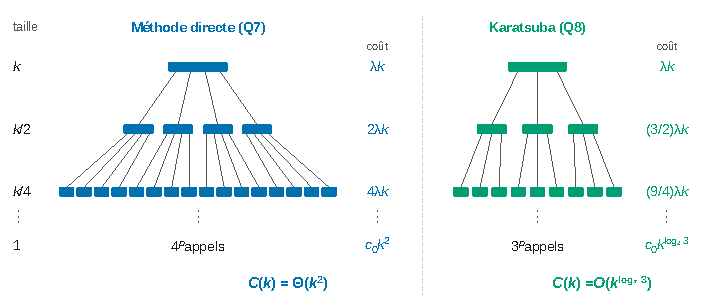
\includegraphics{figures/q8-arbres-appels.pdf}
\caption*{Figure 1 --- Arbres des appels récursifs : chaque niveau coûte deux fois
plus que le précédent avec 4 appels, 3/2 fois plus avec Karatsuba}
\end{figure}

\hypertarget{q9}{%
\subsection{Q9}\label{q9}}

Si \(n = \sum_{j=0}^{k} n_j b^j\), alors

\equationajustee{b^i n = \sum_{j=0}^{k} n_j b^{j+i}.}

Le chiffre de rang \(j\) passe au rang \(j + i\) et les rangs \(0, \dots, i-1\) deviennent nuls. \textbf{Multiplier par \(b^i\) revient à décaler les chiffres de \(i\) rangs vers les poids forts}, c'est-à-dire, avec la convention de l'énoncé (poids faibles en tête), à \textbf{insérer \(i\) zéros en début de liste}. Aucune multiplication n'est effectuée.

\hypertarget{q10}{%
\subsection{Q10}\label{q10}}

\begin{lstlisting}[language=Python]
def shift(lst_bits, i):
    return [0] * i + lst_bits
\end{lstlisting}

L'opérateur \texttt{+} crée une nouvelle liste sans modifier ses opérandes. Le chiffre de rang \(j\) du résultat vaut \(0\) si \(j < i\) et \(n_{j-i}\) sinon : la valeur est \(2^i n\).

Coût \(O(i + \ell)\), où \(\ell\) est la longueur de la liste.

\hypertarget{q11}{%
\subsection{Q11}\label{q11}}

L'énoncé ne prévoit pas que la différence \(f_u - d_u\) puisse être négative, ce qui arrive. On suppose donc d'abord, comme l'impose la formule (2), que \texttt{sub\_bit\_lst} réalise la soustraction sur des entiers relatifs et que son résultat n'est pas plus long que le plus long de ses arguments. Une variante sur les seuls entiers naturels suit.

\begin{lstlisting}[language=Python]
def karatsuba(lst1, lst2):
    n = max(len(lst1), len(lst2))
    lst1 = complement(lst1, n)
    lst2 = complement(lst2, n)
    if n == 0:
        # A : listes vides, le produit vaut 0
        return []
    if n == 1:
        # B : produit de deux bits
        return [lst1[0] * lst2[0]]
    else:
        h = n//2
        d1 = lst1[0:h]
        f1 = lst1[h:]
        d2 = lst2[0:h]
        f2 = lst2[h:]
        # C : trois produits récursifs, puis recollement selon (2)
        p1 = karatsuba(d1, d2)
        p2 = karatsuba(f1, f2)
        p3 = karatsuba(sub_bit_lst(f1, d1), sub_bit_lst(f2, d2))
        m = sub_bit_lst(sum_bit_lst(p2, p1), p3)      # = f1*d2 + d1*f2 >= 0
        return sum_bit_lst(sum_bit_lst(p1, shift(m, h)), shift(p2, 2 * h))
\end{lstlisting}

Justification. Avec \(h = n//2\), \(u = d_1 + b^h f_1\) et \(v = d_2 + b^h f_2\) (même si \(n\) est impair), donc par (2) écrite avec l'exposant \(h\) :

\equationajustee{u \times v = P_1 + b^{h}\,(P_2 + P_1 - P_3) + b^{2h}\,P_2,}

ce que renvoie la partie C.

\begin{itemize}
\tightlist
\item
  Les cas de base renvoient des \textbf{listes} : \texttt{{[}{]}} représente \(0\), et \texttt{{[}x{]}} le produit de deux bits.
\item
  Le \texttt{return} de la partie A est indispensable : sans lui, le cas \(n = 0\) tomberait dans le \texttt{else} avec \(h = 0\), et l'appel \texttt{karatsuba(\allowbreak{}f1,\allowbreak{}\ f2)\allowbreak{}} reboucherait indéfiniment.
\item
  Le décalage du terme de tête est \(2h\) et non \(n\) : les deux diffèrent si \(n\) est impair.
\item
  Terminaison : pour \(n \ge 2\), on a \(1 \le h \le n - 1\). Les trois appels portent sur des listes de longueur au plus \(n - h < n\).
\end{itemize}

Variante n'employant que des entiers naturels (sous-fonctions définies dans la partie C ou au préalable) : on calcule \(|f_1 - d_1|\) et \(|f_2 - d_2|\) après comparaison, et l'on retranche ou ajoute le produit selon les signes.

\begin{lstlisting}[language=Python]
def inferieur(a, b):
    # a < b pour deux listes de bits (comparaison depuis le poids fort)
    n = max(len(a), len(b))
    a = complement(a, n)
    b = complement(b, n)
    for i in range(n - 1, -1, -1):
        if a[i] != b[i]:
            return a[i] < b[i]
    return False

def karatsuba(lst1, lst2):
    n = max(len(lst1), len(lst2))
    lst1 = complement(lst1, n)
    lst2 = complement(lst2, n)
    if n == 0:
        return []
    if n == 1:
        return [lst1[0] * lst2[0]]
    else:
        h = n//2
        d1 = lst1[0:h]
        f1 = lst1[h:]
        d2 = lst2[0:h]
        f2 = lst2[h:]
        # C, version entiers naturels
        p1 = karatsuba(d1, d2)
        p2 = karatsuba(f1, f2)
        neg1 = inferieur(f1, d1)            # f1 - d1 < 0 ?
        neg2 = inferieur(f2, d2)
        if neg1:
            a1 = sub_bit_lst(d1, f1)
        else:
            a1 = sub_bit_lst(f1, d1)
        if neg2:
            a2 = sub_bit_lst(d2, f2)
        else:
            a2 = sub_bit_lst(f2, d2)
        p3 = karatsuba(a1, a2)              # valeur absolue de P3
        if neg1 == neg2:                    # P3 >= 0
            m = sub_bit_lst(sum_bit_lst(p2, p1), p3)
        else:                               # P3 <= 0
            m = sum_bit_lst(sum_bit_lst(p2, p1), p3)
        return sum_bit_lst(sum_bit_lst(p1, shift(m, h)), shift(p2, 2 * h))
\end{lstlisting}

Le nombre d'appels récursifs reste 3 et la comparaison est linéaire : la complexité est inchangée. Cette version a été testée sur 3 000 couples aléatoires d'entiers d'au plus 40 bits et sur \(123\,456\,789 \times 987\,654\,321 = 121\,932\,631\,112\,635\,269\).

\begin{center}\rule{0.5\linewidth}{0.5pt}\end{center}

\hypertarget{probluxe8me-2-ensembles-de-mots-impluxe9mentuxe9s-par-tries}{%
\section{Problème 2 --- Ensembles de mots implémentés par tries}\label{probluxe8me-2-ensembles-de-mots-impluxe9mentuxe9s-par-tries}}

\hypertarget{q12}{%
\subsection{Q12}\label{q12}}

Deux implémentations au programme de la structure de dictionnaire :

\begin{itemize}
\tightlist
\item
  \textbf{les arbres binaires de recherche} (éventuellement équilibrés), les clés étant ordonnées ; recherche, ajout et suppression en \(O(h)\) où \(h\) est la hauteur ;
\item
  \textbf{les tables de hachage}, où une fonction de hachage envoie la clé sur une case d'un tableau ; coût moyen \(O(1)\) par opération sous de bonnes hypothèses de hachage, linéaire dans le pire cas.
\end{itemize}

\hypertarget{q13}{%
\subsection{Q13}\label{q13}}

On prend les mots comme \textbf{clés} du dictionnaire, la valeur associée étant sans importance (par exemple \texttt{true} ou \texttt{()}). Un mot appartient à l'ensemble si et seulement si il est une clé du dictionnaire : le test d'appartenance est une recherche de clé. Avec une table de hachage, il coûte en moyenne le calcul du haché, \(O(|m|)\) ; avec un arbre binaire de recherche équilibré sur l'ordre lexicographique, \(O(|m| \log n)\) pour \(n\) mots.

\hypertarget{q14}{%
\subsection{Q14}\label{q14}}

Le trie de \{en, entier, bot, bottier, bottine, routier, routine\} (la lettre étiquette l'arête qui mène au nœud ; les enfants vides ne sont pas représentés) :

\begin{figure}[H]
\centering
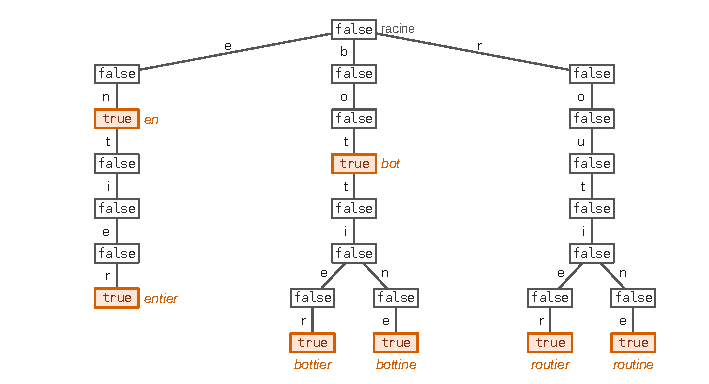
\includegraphics{figures/q14-trie.pdf}
\caption*{Figure 2 --- Trie de l'ensemble en, entier, bot, bottier, bottine,
routier, routine : 25 nœuds, 7 nœuds true, hauteur 7}
\end{figure}

Il compte 25 nœuds, dont 7 marqués \texttt{true} (un par mot), et a pour hauteur 7.

\hypertarget{q15}{%
\subsection{Q15}\label{q15}}

\begin{lstlisting}[language=Caml]
let string_to_list s =
  let n = String.length s in
  (* caracteres_depuis i renvoie la liste des caractères de s
     d'indices i, i+1, ..., n-1 *)
  let rec caracteres_depuis i =
    if i >= n then []
    else s.[i] :: caracteres_depuis (i + 1)
  in
  caracteres_depuis 0
\end{lstlisting}

Rôle de la fonction auxiliaire : \texttt{caracteres\_depuis\ i} renvoie la liste des caractères de \texttt{s} à partir de l'indice \(i\). Par récurrence descendante sur \(i\), elle vaut \texttt{{[}s.{[}i{]}\allowbreak{};\allowbreak{}\ ...;\allowbreak{}\ s.{[}n-1{]}\allowbreak{}{]}\allowbreak{}} : c'est vrai pour \(i = n\), et si c'est vrai pour \(i+1\), c'est vrai pour \(i\).

Complexité : \texttt{String.length} est appelée une fois, en \(O(1)\). Il y a \(n + 1\) appels à \texttt{caracteres\_depuis}, chacun en \(O(1)\) (comparaison, accès \texttt{s.{[}i{]}}, construction \texttt{::} en tête). \textbf{Le coût est \(O(n)\)}, où \(n\) est la longueur de la chaîne. Aucune concaténation \texttt{@}, dont le coût est linéaire en la longueur de son premier argument, n'est utilisée.

\texttt{string\_to\_list\ "lettre"} vaut \texttt{{[}\textquotesingle{}l\textquotesingle{};\allowbreak{}\ \textquotesingle{}e\textquotesingle{};\allowbreak{}\ \textquotesingle{}t\textquotesingle{};\allowbreak{}\ \textquotesingle{}t\textquotesingle{};\allowbreak{}\ \textquotesingle{}r\textquotesingle{};\allowbreak{}\ \textquotesingle{}e\textquotesingle{}{]}\allowbreak{}}.

\hypertarget{q16}{%
\subsection{Q16}\label{q16}}

Le type n'a pas de constructeur vide : le plus petit trie est une racine sans enfant, marquée \texttt{false}. Marquée \texttt{true}, elle représenterait l'ensemble réduit au mot vide, et non l'ensemble vide.

\begin{lstlisting}[language=Caml]
let empty_trie () = Node (false, [])
\end{lstlisting}

C'est bien une fonction de type \texttt{unit\ -\textgreater{}\ trie}, comme demandé, et non une constante de type \texttt{trie}.

\hypertarget{q17}{%
\subsection{Q17}\label{q17}}

\begin{lstlisting}[language=Caml]
let rec max_list lst =
  match lst with
  | [] -> failwith "max_list : liste vide"
  | [x] -> x
  | x :: reste ->
      let m = max_list reste in
      if x > m then x else m
\end{lstlisting}

Par récurrence sur la longueur \(\ell \ge 1\) : pour \(\ell = 1\) on renvoie l'unique élément ; sinon \(m\) est le maximum de \texttt{reste} et le maximum de la liste est \(\max(x, m)\). Un seul appel récursif par élément (grâce au \texttt{let}) : coût linéaire. La fonction est directement récursive : aucun accumulateur n'est à initialiser, et rien n'est supposé sur le signe des éléments.

\hypertarget{q18}{%
\subsection{Q18}\label{q18}}

\begin{lstlisting}[language=Caml]
let rec list_map f lst =
  match lst with
  | [] -> []
  | x :: reste -> f x :: list_map f reste
\end{lstlisting}

Par récurrence immédiate, \texttt{list\_map\ f\ {[}x1;\allowbreak{}\ ...;\allowbreak{}\ xn{]}\allowbreak{}} vaut \texttt{{[}f\ x1;\allowbreak{}\ ...;\allowbreak{}\ f\ xn{]}\allowbreak{}}, dans le même ordre ; le type inféré est \texttt{(\allowbreak{}\textquotesingle{}a\ -\textgreater{}\ \textquotesingle{}b)\allowbreak{}\ -\textgreater{}\ \textquotesingle{}a\ list\ -\textgreater{}\ \textquotesingle{}b\ list}.

\hypertarget{q19}{%
\subsection{Q19}\label{q19}}

Convention : la hauteur est le nombre d'arêtes du plus long chemin de la racine à une feuille ; un nœud seul est de hauteur 0.

\begin{lstlisting}[language=Caml]
let rec height t =
  match t with
  | Node (_, []) -> 0
  | Node (_, enfants) ->
      1 + max_list (list_map (fun (_, fils) -> height fils) enfants)
\end{lstlisting}

Si le nœud a des enfants \(t_1, \dots, t_p\) (\(p \ge 1\)), la hauteur vaut \(1 + \max_j \mathrm{hauteur}(t_j)\), et la liste passée à \texttt{max\_list} est non vide. Les enfants sont des couples (lettre, sous-trie) : la fonction passée à \texttt{list\_map} ignore la lettre. Sur le trie de Q14, \texttt{height} vaut 7.

\hypertarget{q20}{%
\subsection{Q20}\label{q20}}

\begin{lstlisting}[language=Caml]
let rec somme_liste lst =
  match lst with
  | [] -> 0
  | x :: reste -> x + somme_liste reste

let rec size t =
  match t with
  | Node (_, enfants) ->
      1 + somme_liste (list_map (fun (_, fils) -> size fils) enfants)
\end{lstlisting}

Par induction structurelle : \texttt{list\_map} calcule la liste des tailles des sous-tries (en ignorant la lettre de chaque couple), \texttt{somme\_liste} les additionne et \texttt{size} ajoute la racine. Une feuille donne \texttt{1\ +\ somme\_liste\ {[}{]}\allowbreak{}}, soit 1. Chaque nœud est visité une fois : coût linéaire en le nombre de nœuds. Sur le trie de Q14, \texttt{size} vaut 25.

\hypertarget{q21}{%
\subsection{Q21}\label{q21}}

Montrons par induction que, pour \(t = \texttt{Node}(b, [(c_1, t_1); \dots; (c_p, t_p)])\),

\equationajustee{f(t) = [b] + \sum_{j=1}^{p} f(t_j),}

où \([b]\) vaut \(1\) si \(b\) est \texttt{true} et \(0\) sinon.

Pour \(p = 0\), les deux premiers cas donnent \(1\) si \(b\) est vrai et \(0\) sinon. Pour \(p \ge 1\), le troisième cas donne

\equationajustee{f(t) = f(t_1) + f(\texttt{Node}(b, [(c_2, t_2); \dots; (c_p, t_p)])).}

Une récurrence sur \(p\) (à \(b\) fixé) donne la formule : le booléen \(b\) n'est examiné qu'une fois, quand la liste est épuisée. Le nœud fictif \texttt{Node\ (b,\ tail)} sert seulement à parcourir la liste des enfants.

Ainsi \(f(t)\) est \textbf{le nombre de nœuds marqués \texttt{true}}, qu'ils soient feuilles ou nœuds internes (comme celui de « le » dans la figure 1). Comme chaque nœud est atteint par un unique chemin depuis la racine, ces nœuds sont en bijection avec les mots du trie :

\textbf{\(f\) calcule le nombre de mots contenus dans le trie} (4 pour la figure 1, 3 pour la figure 2, 7 pour le trie de Q14).

\hypertarget{q22}{%
\subsection{Q22}\label{q22}}

\begin{lstlisting}[language=Caml]
let rec is_in_trie mot t =
  match mot, t with
  | [], Node (b, _) -> b
  | c :: reste, Node (_, enfants) -> is_in_children c reste enfants
and is_in_children c reste enfants =
  match enfants with
  | [] -> false
  | (l, fils) :: suite ->
      if l = c then is_in_trie reste fils
      else is_in_children c reste suite
\end{lstlisting}

Mot vide : il est dans le trie si et seulement si la racine porte \texttt{true}. Mot \(c \cdot w\) : il y est si et seulement si la racine a un enfant étiqueté \(c\) dont le sous-trie contient \(w\) ; s'il n'y a pas d'enfant \(c\), c'est un enfant vide et la réponse est \texttt{false}. Coût \(O(|m| \cdot |\Sigma|)\).

\hypertarget{q23}{%
\subsection{Q23}\label{q23}}

\begin{lstlisting}[language=Caml]
let rec add_to_trie mot t =
  match mot, t with
  | [], Node (_, enfants) -> Node (true, enfants)
  | c :: reste, Node (b, enfants) -> Node (b, add_children c reste enfants)
and add_children c reste enfants =
  match enfants with
  | [] -> [(c, add_to_trie reste (empty_trie ()))]
  | (l, fils) :: suite ->
      if l = c then (l, add_to_trie reste fils) :: suite
      else (l, fils) :: add_children c reste suite
\end{lstlisting}

Algorithme. Un trie n'est pas modifiable en place : on renvoie un nouveau trie, en reconstruisant les nœuds le long du chemin étiqueté par le mot et en partageant tous les autres sous-tries.

Mot vide : on marque la racine en \textbf{conservant ses enfants} (on ne perd aucun mot dont le mot ajouté est préfixe). Mot \(c \cdot w\) : on ajoute \(w\) dans le sous-trie d'étiquette \(c\) s'il existe, sinon on crée une branche à partir du trie vide ; les autres enfants et le booléen sont conservés. L'ensemble des mots du résultat est l'ensemble initial augmenté du mot. Testé : en insérant les sept mots de Q14 dans \texttt{empty\_trie\ ()}, on obtient un trie de taille 25, de hauteur 7, où \texttt{f} vaut 7 ; les sept mots sont reconnus, et \texttt{e}, \texttt{ent}, \texttt{bo}, \texttt{rout} ne le sont pas.

\hypertarget{q24}{%
\subsection{Q24}\label{q24}}

Un trie partage les \textbf{préfixes} communs mais \textbf{pas les suffixes}. Sur l'exemple de Q14, les sous-arbres issus de \texttt{botti} et de \texttt{routi} sont identiques (ils codent les suffixes \{er, ne\}) et sont stockés deux fois ; la branche finale \texttt{e\ →\ r} apparaît trois fois (sous \texttt{enti}, \texttt{botti}, \texttt{routi}). La taille du trie est de l'ordre du nombre total de lettres des mots, diminué des seuls préfixes communs : pour un lexique riche en terminaisons communes (pluriels, conjugaisons), \textbf{la structure contient de nombreux sous-arbres identiques, redondants}, ce qui gaspille de la mémoire (le temps de recherche, lui, reste en \(O(|m|)\)).

\hypertarget{q25}{%
\subsection{Q25}\label{q25}}

À un trie, on associe l'automate fini \((\Sigma, Q, I, F, \delta)\) :

\begin{itemize}
\tightlist
\item
  \textbf{alphabet} \(\Sigma\) : l'ensemble des lettres (celles qui étiquettent les arêtes) ;
\item
  \textbf{états} \(Q\) : les nœuds du trie ;
\item
  \textbf{état initial} : la racine (unique) ;
\item
  \textbf{états finaux} \(F\) : les nœuds portant \texttt{true} ;
\item
  \textbf{transitions} : les triplets \((q, c, q')\) où \(q'\) est l'enfant de \(q\) étiqueté \(c\), soit \(\delta(q, c) = q'\) ; pas de transition (blocage) si cet enfant est vide.
\end{itemize}

L'automate est déterministe, en général incomplet, et acyclique. Lire un mot depuis la racine suit l'unique chemin qu'il étiquette ; il est accepté si et seulement si le nœud atteint porte \texttt{true} : le langage reconnu est l'ensemble des mots du trie.

\hypertarget{q26}{%
\subsection{Q26}\label{q26}}

On note \(q_w\) l'état atteint en lisant \(w\) depuis l'état initial \(q_\varepsilon\). L'automate a \textbf{25 états et 24 transitions} (une par arête du trie). Chaque transition est orientée vers l'enfant ; les états finaux sont doublement cerclés et la flèche entrante marque l'état initial :

\begin{figure}[H]
\centering
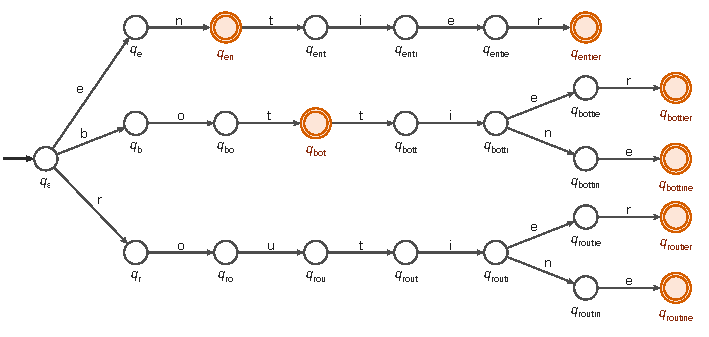
\includegraphics{figures/q26-automate-trie.pdf}
\caption*{Figure 3 --- Automate du trie de Q14 : état initial q\_ε, états finaux
doublement cerclés, 25 états et 24 transitions}
\end{figure}

États finaux : \(q_{en},\allowbreak q_{entier},\allowbreak q_{bot},\allowbreak q_{bottier},\allowbreak q_{bottine},\allowbreak q_{routier},\allowbreak q_{routine}\). Le dessin est celui du trie de Q14, avec des flèches orientées vers les enfants ; aucun état n'est fusionné à ce stade.

\hypertarget{q27}{%
\subsection{Q27}\label{q27}}

\textbf{Sans transition sortante} : \(q_{bottier}\) et \(q_{routier}\). Ils sont tous deux finaux, et toute lettre est un blocage pour les deux. Donc \(q_{bottier}\, E\, q_{routier}\) (de même pour tout couple pris parmi \(q_{entier},\allowbreak q_{bottier},\allowbreak q_{bottine},\allowbreak q_{routier},\allowbreak q_{routine}\)).

\textbf{Avec transition sortante} : \(q_{bottie}\) et \(q_{routie}\). Ils sont tous deux non finaux ; pour la lettre \texttt{r}, \(\delta(q_{bottie}, r) = q_{bottier}\) et \(\delta(q_{routie}, r) = q_{routier}\), en relation d'après ce qui précède ; toute autre lettre bloque pour les deux. Donc \(q_{bottie}\, E\, q_{routie}\).

\hypertarget{q28}{%
\subsection{Q28}\label{q28}}

\textbf{Démarche.} \(E\) est une relation d'équivalence (réflexivité, symétrie et transitivité se vérifient par récurrence sur la hauteur des états, l'automate étant acyclique). On fusionne chaque classe en un seul état (\textbf{automate quotient}) :

\begin{itemize}
\tightlist
\item
  états : les classes \([q]\) ; état initial : \([q_\varepsilon]\) ;
\item
  \([q]\) est final si \(q\) l'est : c'est bien défini car deux états en relation ont même finalité ;
\item
  \(\delta'([q], c) = [\delta(q, c)]\) si \(\delta(q, c)\) existe : bien défini car si \(q\,E\,q'\), la lettre \(c\) bloque pour les deux ou \(\delta(q, c)\, E\, \delta(q', c)\).
\end{itemize}

Deux états en relation reconnaissant le même langage (résultat admis), la fusion ne change pas le langage reconnu. Calcul effectif, de bas en haut : on traite les états par hauteur croissante (longueur du plus long chemin qui en part). À chaque état on associe sa \textbf{signature} : sa finalité et l'ensemble des couples \((c, [\delta(q, c)])\) pour les lettres non bloquantes, les classes des successeurs étant déjà connues. Deux états sont en relation si et seulement si ils ont même signature ; on regroupe les états par signature. Le résultat n'est plus un arbre : les suffixes communs sont partagés.

\textbf{Illustration sur \{car, par, cal, pal\}.} L'automate du trie a 9 états : \(q_\varepsilon,\allowbreak q_c,\allowbreak q_{ca},\allowbreak q_{car},\allowbreak q_{cal},\allowbreak q_p,\allowbreak q_{pa},\allowbreak q_{par},\allowbreak q_{pal}\).

\begin{longtable}[]{@{}
  >{\raggedright\arraybackslash}p{(\columnwidth - 6\tabcolsep) * \real{0.2500}}
  >{\raggedright\arraybackslash}p{(\columnwidth - 6\tabcolsep) * \real{0.2500}}
  >{\raggedright\arraybackslash}p{(\columnwidth - 6\tabcolsep) * \real{0.2500}}
  >{\raggedright\arraybackslash}p{(\columnwidth - 6\tabcolsep) * \real{0.2500}}@{}}
\toprule\noalign{}
\begin{minipage}[b]{\linewidth}\raggedright
Hauteur
\end{minipage} & \begin{minipage}[b]{\linewidth}\raggedright
États
\end{minipage} & \begin{minipage}[b]{\linewidth}\raggedright
Signature
\end{minipage} & \begin{minipage}[b]{\linewidth}\raggedright
Classe
\end{minipage} \\
\midrule\noalign{}
\endhead
\bottomrule\noalign{}
\endlastfoot
0 & \(q_{car}, q_{cal}, q_{par}, q_{pal}\) & final, aucune transition & \(X\) \\
1 & \(q_{ca}, q_{pa}\) & non final, r → \(X\), l → \(X\) & \(Y\) \\
2 & \(q_c, q_p\) & non final, a → \(Y\) & \(Z\) \\
3 & \(q_\varepsilon\) & non final, c → \(Z\), p → \(Z\) & \(R\) \\
\end{longtable}

L'automate simplifié a \textbf{4 états au lieu de 9} :

\begin{figure}[H]
\centering
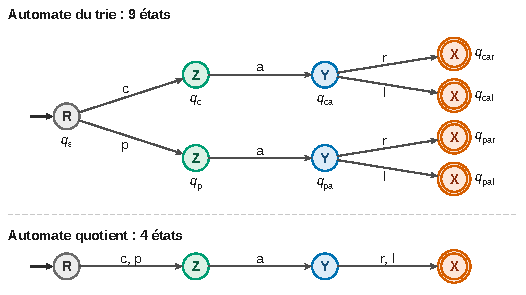
\includegraphics{figures/q28-minimisation.pdf}
\caption*{Figure 4 --- Minimisation pour car, par, cal, pal : les états de même
classe fusionnent, de 9 à 4 états}
\end{figure}

Il reconnaît \(\{c, p\} \cdot \{a\} \cdot \{r, l\} = \{car, cal, par, pal\}\).

Appliquée au trie de Q14, la même démarche fusionne successivement :

\begin{itemize}
\tightlist
\item
  les cinq états finaux sans successeur ;
\item
  \(q_{entie}, q_{bottie}, q_{routie}\) ;
\item
  \(q_{bottin}\) et \(q_{routin}\) ;
\item
  \(q_{botti}\) et \(q_{routi}\) ;
\item
  \(q_{bott}\) et \(q_{rout}\).
\end{itemize}

On passe de 25 à 16 états.

\begin{center}\rule{0.5\linewidth}{0.5pt}\end{center}

\hypertarget{probluxe8me-3-logique-implicationnelle}{%
\section{Problème 3 --- Logique implicationnelle}\label{probluxe8me-3-logique-implicationnelle}}

Notations. Les valeurs de vérité sont notées V et F ; \(\top\) et \(\bot\) désignent des formules.

\begin{itemize}
\tightlist
\item
  Une valuation \(v\) s'étend aux formules par les tables de vérité, avec \(v(\top) = V\) et \(v(\bot) = F\).
\item
  \(A \equiv B\) signifie \(v(A) = v(B)\) pour toute valuation \(v\).
\item
  \(\Gamma \models F\) (conséquence sémantique) signifie que toute valuation satisfaisant toutes les formules de \(\Gamma\) satisfait \(F\).
\end{itemize}

La valeur d'une formule construite par un connecteur ne dépend que des valeurs de ses sous-formules. On peut donc remplacer une sous-formule par une formule équivalente (\textbf{lemme de remplacement}).

\hypertarget{q29}{%
\subsection{Q29}\label{q29}}

\begin{longtable}[]{@{}lllll@{}}
\toprule\noalign{}
\(v(A)\) & \(v(B)\) & \(A \to B\) & \(\neg A\) & \(\neg A \vee B\) \\
\midrule\noalign{}
\endhead
\bottomrule\noalign{}
\endlastfoot
V & V & V & F & V \\
V & F & F & F & F \\
F & V & V & V & V \\
F & F & V & V & V \\
\end{longtable}

Pour toute valuation, \((v(A), v(B))\) est l'une des quatre lignes, et les deux dernières colonnes coïncident : \(\boxed{A \to B \equiv \neg A \vee B}\).

\hypertarget{q30}{%
\subsection{Q30}\label{q30}}

\begin{longtable}[]{@{}llll@{}}
\toprule\noalign{}
\(v(A)\) & \(\bot\) & \(A \to \bot\) & \(\neg A\) \\
\midrule\noalign{}
\endhead
\bottomrule\noalign{}
\endlastfoot
V & F & F & F \\
F & F & V & V \\
\end{longtable}

\textbf{Oui} : \(\boxed{\neg A \equiv A \to \bot}\). On le retrouve aussi par Q29 : \(A \to \bot \equiv \neg A \vee \bot\), qui a la valeur de \(\neg A\).

\hypertarget{q31}{%
\subsection{Q31}\label{q31}}

\begin{longtable}[]{@{}
  >{\raggedright\arraybackslash}p{(\columnwidth - 8\tabcolsep) * \real{0.2000}}
  >{\raggedright\arraybackslash}p{(\columnwidth - 8\tabcolsep) * \real{0.2000}}
  >{\raggedright\arraybackslash}p{(\columnwidth - 8\tabcolsep) * \real{0.2000}}
  >{\raggedright\arraybackslash}p{(\columnwidth - 8\tabcolsep) * \real{0.2000}}
  >{\raggedright\arraybackslash}p{(\columnwidth - 8\tabcolsep) * \real{0.2000}}@{}}
\toprule\noalign{}
\begin{minipage}[b]{\linewidth}\raggedright
\(v(A)\)
\end{minipage} & \begin{minipage}[b]{\linewidth}\raggedright
\(v(B)\)
\end{minipage} & \begin{minipage}[b]{\linewidth}\raggedright
\(A \to B\)
\end{minipage} & \begin{minipage}[b]{\linewidth}\raggedright
\((A \to B) \to A\)
\end{minipage} & \begin{minipage}[b]{\linewidth}\raggedright
\(\varphi\)
\end{minipage} \\
\midrule\noalign{}
\endhead
\bottomrule\noalign{}
\endlastfoot
V & V & V & V & V \\
V & F & F & V & V \\
F & V & V & F & V \\
F & F & V & F & V \\
\end{longtable}

La dernière colonne ne contient que V : \(\varphi\) est vraie sous toute valuation, c'est-à-dire que \textbf{\(\varphi\) est une tautologie} (loi de Peirce).

\hypertarget{q32}{%
\subsection{Q32}\label{q32}}

Équivalences préalables (vérifiées par table de vérité) :

\begin{longtable}[]{@{}
  >{\raggedright\arraybackslash}p{(\columnwidth - 10\tabcolsep) * \real{0.1667}}
  >{\raggedright\arraybackslash}p{(\columnwidth - 10\tabcolsep) * \real{0.1667}}
  >{\raggedright\arraybackslash}p{(\columnwidth - 10\tabcolsep) * \real{0.1667}}
  >{\raggedright\arraybackslash}p{(\columnwidth - 10\tabcolsep) * \real{0.1667}}
  >{\raggedright\arraybackslash}p{(\columnwidth - 10\tabcolsep) * \real{0.1667}}
  >{\raggedright\arraybackslash}p{(\columnwidth - 10\tabcolsep) * \real{0.1667}}@{}}
\toprule\noalign{}
\begin{minipage}[b]{\linewidth}\raggedright
\(v(A)\)
\end{minipage} & \begin{minipage}[b]{\linewidth}\raggedright
\(v(B)\)
\end{minipage} & \begin{minipage}[b]{\linewidth}\raggedright
\(A \vee B\)
\end{minipage} & \begin{minipage}[b]{\linewidth}\raggedright
\(\neg A \to B\)
\end{minipage} & \begin{minipage}[b]{\linewidth}\raggedright
\(A \wedge B\)
\end{minipage} & \begin{minipage}[b]{\linewidth}\raggedright
\(\neg(A \to \neg B)\)
\end{minipage} \\
\midrule\noalign{}
\endhead
\bottomrule\noalign{}
\endlastfoot
V & V & V & V & V & V \\
V & F & V & V & F & F \\
F & V & V & V & F & F \\
F & F & F & F & F & F \\
\end{longtable}

donc \(A \vee B \equiv \neg A \to B\) et \(A \wedge B \equiv \neg(A \to \neg B)\).

\textbf{Propriété démontrée.} Pour \(F \in S_P\), on note \(\mathcal{P}(F)\) la propriété : « il existe une formule \(F'\), équivalente à \(F\), dont les seuls connecteurs sont \(\neg\) et \(\to\) ».

Montrons \(\mathcal{P}(F)\) pour toute \(F \in S_P\), par induction structurelle sur \(F\) (et non par récurrence sur sa taille).

\textbf{Cas de base.} Si \(F\) est \(\top\), \(\bot\) ou une variable propositionnelle \(p\), la formule \(F' = F\) ne contient aucun connecteur : \(\mathcal{P}(F)\) est vraie.

\textbf{Cas inductifs.} Soient \(A\) et \(B\) deux formules vérifiant \(\mathcal{P}\) (hypothèse d'induction).

On fixe donc \(A' \equiv A\) et \(B' \equiv B\), deux formules n'utilisant que \(\neg\) et \(\to\).

\begin{itemize}
\tightlist
\item
  \(F = \neg A\). Par le lemme de remplacement appliqué à \(A \equiv A'\), on a \(F \equiv \neg A'\), formule qui n'utilise que \(\neg\) et \(\to\).
\item
  \(F = A \to B\). Par remplacement de \(A\) et \(B\), on a \(F \equiv A' \to B'\).
\item
  \(F = A \vee B\). Par remplacement, puis par l'équivalence préalable appliquée à \(A'\) et \(B'\) :
\end{itemize}

\equationajustee{\begin{aligned}
F &\equiv A' \vee B' \\
&\equiv \neg A' \to B'.
\end{aligned}}

\begin{itemize}
\tightlist
\item
  \(F = A \wedge B\). De même :
\end{itemize}

\equationajustee{\begin{aligned}
F &\equiv A' \wedge B' \\
&\equiv \neg(A' \to \neg B').
\end{aligned}}

Dans chacun des quatre cas, la formule obtenue n'utilise que \(\neg\) et \(\to\), puisque \(A'\) et \(B'\) n'utilisent qu'eux : \(\mathcal{P}(F)\) est vraie.

\textbf{Conclusion.} Par induction structurelle, \(\mathcal{P}(F)\) est vraie pour toute formule de \(S_P\). \textbf{Le système \(\{\neg, \to\}\) est complet.}

\hypertarget{q33}{%
\subsection{Q33}\label{q33}}

Soit \(F \in S_P\). Par Q32, \(F \equiv F'\) où \(F'\) n'utilise que \(\neg\) et \(\to\).

Par induction structurelle sur \(F'\), construisons une formule de \(S_I\) équivalente :

\begin{itemize}
\tightlist
\item
  \(\top\), \(\bot\), variable : déjà dans \(S_I\) ;
\item
  \(A \to B\) : avec \(A''\) et \(B''\) données par l'hypothèse d'induction, \(A \to B \equiv A'' \to B''\), qui est dans \(S_I\) ;
\item
  \(\neg A\) : par remplacement puis par Q30,
\end{itemize}

\equationajustee{\begin{aligned}
\neg A &\equiv \neg A'' \\
&\equiv A'' \to \bot,
\end{aligned}}

et \(A'' \to \bot\) est dans \(S_I\).

Par transitivité de \(\equiv\), \(F\) est équivalente à une formule \(F''\) de \(S_I\).

\textbf{Toute formule de \(S_P\) est équivalente à une formule de \(S_I\).} La présence de \(\bot\) dans \(S_I\) est essentielle pour exprimer la négation.

\hypertarget{q34}{%
\subsection{Q34}\label{q34}}

\textbf{1.} \(A \vdash (A \to B) \to B\). On note \(\Gamma_1 = A, A \to B\).

\equationajustee{\dfrac{\dfrac{\dfrac{}{\Gamma_1 \vdash A \to B}\,\text{ax} \qquad \dfrac{}{\Gamma_1 \vdash A}\,\text{ax}}{\Gamma_1 \vdash B}\,\text{elim-}\to}{A \vdash (A \to B) \to B}\,\text{intro-}\to}

\textbf{2.} \(A \to B, B \to C \vdash A \to C\). On note \(\Gamma_2 = A \to B, B \to C, A\).

\equationajustee{\dfrac{\dfrac{\dfrac{}{\Gamma_2 \vdash B \to C}\,\text{ax} \qquad \dfrac{\dfrac{}{\Gamma_2 \vdash A \to B}\,\text{ax} \qquad \dfrac{}{\Gamma_2 \vdash A}\,\text{ax}}{\Gamma_2 \vdash B}\,\text{elim-}\to}{\Gamma_2 \vdash C}\,\text{elim-}\to}{A \to B, B \to C \vdash A \to C}\,\text{intro-}\to}

\textbf{3.} \((A \to B) \to C, A \to C \vdash C\). On note \(\Gamma_3 = (A \to B) \to C, A \to C\) et \(\Delta = \Gamma_3, C \to B\).

Dans \(\Delta\), on obtient \(A \to B\) comme au point 2, à partir de \(A \to C\) et de \(C \to B\) (arbre \(\pi\), utilisé plus bas) :

\equationajustee{\pi = \dfrac{\dfrac{\dfrac{}{\Delta, A \vdash C \to B}\,\text{ax} \qquad \dfrac{\dfrac{}{\Delta, A \vdash A \to C}\,\text{ax} \qquad \dfrac{}{\Delta, A \vdash A}\,\text{ax}}{\Delta, A \vdash C}\,\text{elim-}\to}{\Delta, A \vdash B}\,\text{elim-}\to}{\Delta \vdash A \to B}\,\text{intro-}\to}

puis, avec l'instance de Peirce \(((C \to B) \to C) \to C\) :

\equationajustee{\dfrac{\dfrac{}{\Gamma_3 \vdash ((C \to B) \to C) \to C}\,\text{Peirce} \qquad \dfrac{\dfrac{\dfrac{}{\Delta \vdash (A \to B) \to C}\,\text{ax} \qquad \overset{\pi}{\Delta \vdash A \to B}}{\Delta \vdash C}\,\text{elim-}\to}{\Gamma_3 \vdash (C \to B) \to C}\,\text{intro-}\to}{\Gamma_3 \vdash C}\,\text{elim-}\to}

\hypertarget{q35}{%
\subsection{Q35}\label{q35}}

Une règle de prémisses \(\Gamma_1 \vdash F_1, \dots, \Gamma_k \vdash F_k\) et de conclusion \(\Gamma \vdash F\) est \textbf{correcte} si : dès que \(\Gamma_i \models F_i\) pour tout \(i\), on a \(\Gamma \models F\). Pour une règle sans prémisse, cela signifie \(\Gamma \models F\).

\begin{itemize}
\tightlist
\item
  \textbf{ax} : toute valuation satisfaisant \(\Gamma \cup \{A\}\) satisfait \(A\), donc \(\Gamma, A \models A\).
\item
  \textbf{Peirce} : la formule est une tautologie (Q31, valable pour des formules \(A\) et \(B\) quelconques). Elle est donc satisfaite par toute valuation, en particulier par celles qui satisfont \(\Gamma\).
\item
  \textbf{elim-\(\to\)} : supposons \(\Gamma \models A \to B\) et \(\Gamma \models A\). Soit \(v\) une valuation satisfaisant \(\Gamma\).
  Elle vérifie \(v(A \to B) = V\) et \(v(A) = V\), donc \(v(B) = V\) par la table de \(\to\).
\item
  \textbf{intro-\(\to\)} : supposons \(\Gamma, A \models B\) et soit \(v\) satisfaisant \(\Gamma\).

  \begin{itemize}
  \tightlist
  \item
    Si \(v(A) = F\), alors \(v(A \to B) = V\).
  \item
    Si \(v(A) = V\), alors \(v\) satisfait \(\Gamma \cup \{A\}\), donc \(v(B) = V\) et \(v(A \to B) = V\).
  \end{itemize}

  Ainsi \(\Gamma \models A \to B\).
\end{itemize}

\textbf{Les quatre règles de \(D_I\) sont correctes.}

\hypertarget{q36}{%
\subsection{Q36}\label{q36}}

On a \(\boxed{\Gamma \models F}\) : \(F\) est conséquence sémantique de \(\Gamma\).

Preuve par induction sur l'arbre de preuve. Si la dernière règle est sans prémisse, sa correction donne directement \(\Gamma \models F\). Sinon, l'hypothèse d'induction s'applique aux sous-arbres : chaque prémisse \(\Gamma_i \vdash F_i\) vérifie \(\Gamma_i \models F_i\). La correction de la dernière règle donne alors \(\Gamma \models F\).

\hypertarget{q37}{%
\subsection{Q37}\label{q37}}

L'arbre prétend prouver \(\Gamma \vdash A \to C\), avec \(\Gamma = \{A \to B, C \to B\}\), en n'utilisant que les règles ax, elim-\(\to\) et intro-\(\to\), toutes correctes (Q35). Raisonnons par l'absurde : s'il était une preuve, Q36 donnerait \(\Gamma \models A \to C\).

Considérons la valuation définie par \(v(A) = V\), \(v(B) = V\) et \(v(C) = F\).

\begin{itemize}
\tightlist
\item
  Elle satisfait \(A \to B\) (conséquent vrai) et \(C \to B\) (antécédent faux) : elle satisfait \(\Gamma\).
\item
  Elle donne \(v(A \to C) = F\).
\end{itemize}

Donc \(\Gamma \not\models A \to C\), ce qui contredit Q36 : \textbf{l'arbre est incorrect}.

L'argument sémantique suffit. On peut ensuite localiser la faute : l'étape qui déduit \(\Gamma, A \vdash C\) de \(\Gamma, A \vdash B\) et \(\Gamma, A \vdash C \to B\) n'est pas une instance de elim-\(\to\).

Cette règle tire \(B\) de \(C \to B\) et de \(C\), pas l'inverse.

\hypertarget{q38}{%
\subsection{Q38}\label{q38}}

On note \(\Gamma = (A \to B) \to A, \neg A\).

\equationajustee{\dfrac{\dfrac{}{\Gamma \vdash (A \to B) \to A}\,\text{ax} \qquad \dfrac{\dfrac{\dfrac{\dfrac{}{\Gamma, A \vdash A}\,\text{ax} \qquad \dfrac{}{\Gamma, A \vdash \neg A}\,\text{ax}}{\Gamma, A \vdash \bot}\,\text{elim-}\neg}{\Gamma, A \vdash B}\,\text{elim-}\bot}{\Gamma \vdash A \to B}\,\text{intro-}\to}{\Gamma \vdash A}\,\text{elim-}\to}

\hypertarget{q39}{%
\subsection{Q39}\label{q39}}

La loi de Peirce est une règle sans prémisse : il faut prouver \(\Gamma \vdash ((A \to B) \to A) \to A\) dans \(D_P\) pour tout contexte \(\Gamma\). Posons \(\Gamma' = \Gamma, (A \to B) \to A\).

L'arbre \(\pi_{38}\) de Q38 n'utilise ax que sur \((A \to B) \to A\), \(\neg A\) et \(A\). Comme la règle ax admet un contexte quelconque, il prouve aussi \(\Gamma', \neg A \vdash A\). Alors :

\equationajustee{\dfrac{\dfrac{\dfrac{\overset{\pi_{38}}{\Gamma', \neg A \vdash A} \qquad \dfrac{}{\Gamma', \neg A \vdash \neg A}\,\text{ax}}{\Gamma', \neg A \vdash \bot}\,\text{elim-}\neg}{\Gamma' \vdash A}\,\text{ra}}{\Gamma \vdash ((A \to B) \to A) \to A}\,\text{intro-}\to}

Toutes les règles employées sont dans \(D_P\) : \textbf{la loi de Peirce est dérivable dans \(D_P\)}.

\hypertarget{q40}{%
\subsection{Q40}\label{q40}}

On suppose une preuve de la prémisse \(\Gamma, \neg A \vdash \bot\) et l'on construit, dans \(D\), une preuve de \(\Gamma \vdash A\). Posons \(\Gamma' = \Gamma, A \to \bot\).

\emph{Étape 1} : \(\Gamma \vdash \neg\neg A\) par intro-\(\neg\) appliquée à la prémisse, puis \(\Gamma' \vdash \neg\neg A\) par affaiblissement.

\emph{Étape 2} : \(\Gamma' \vdash \neg A\) :

\equationajustee{\dfrac{\dfrac{\dfrac{}{\Gamma', A \vdash A \to \bot}\,\text{ax} \qquad \dfrac{}{\Gamma', A \vdash A}\,\text{ax}}{\Gamma', A \vdash \bot}\,\text{elim-}\to}{\Gamma' \vdash \neg A}\,\text{intro-}\neg}

\emph{Étape 3} : elim-\(\neg\) (appliquée à la formule \(\neg A\)) puis elim-\(\bot\) :

\equationajustee{\dfrac{\dfrac{\Gamma' \vdash \neg A \qquad \Gamma' \vdash \neg\neg A}{\Gamma' \vdash \bot}\,\text{elim-}\neg}{\Gamma' \vdash A}\,\text{elim-}\bot}

\emph{Étape 4} : intro-\(\to\) et l'instance de Peirce \(((A \to \bot) \to A) \to A\) :

\equationajustee{\dfrac{\dfrac{}{\Gamma \vdash ((A \to \bot) \to A) \to A}\,\text{Peirce} \qquad \dfrac{\Gamma' \vdash A}{\Gamma \vdash (A \to \bot) \to A}\,\text{intro-}\to}{\Gamma \vdash A}\,\text{elim-}\to}

Seules des règles de \(D\) ont été utilisées, jamais ra :

\begin{itemize}
\tightlist
\item
  ax, aff et Peirce ;
\item
  intro-\(\neg\), elim-\(\neg\) et elim-\(\bot\) ;
\item
  intro-\(\to\) et elim-\(\to\).
\end{itemize}

Le passage de \(A \to \bot\) à \(\neg A\) se fait par des règles (étape 2), et non par l'équivalence sémantique de Q30. \textbf{Le raisonnement par l'absurde est dérivable dans \(D\).}

\hypertarget{q41}{%
\subsection{Q41}\label{q41}}

\textbf{\(D\) et \(D_P\) prouvent exactement les mêmes séquents.} En effet, ils ont les mêmes règles hormis ra (dans \(D_P\)) et Peirce (dans \(D\)).

\begin{itemize}
\tightlist
\item
  Dans un arbre de preuve de \(D\), on remplace chaque feuille Peirce par la dérivation de Q39 : on obtient une preuve dans \(D_P\).
\item
  Dans un arbre de preuve de \(D_P\), on remplace chaque application de ra par le fragment de Q40, greffé sur la preuve (déjà traduite) de sa prémisse : on obtient une preuve dans \(D\), par induction sur l'arbre de preuve.
\end{itemize}

Ainsi \(D\) est une autre présentation de la déduction naturelle classique : la loi de Peirce peut remplacer le raisonnement par l'absurde. En particulier, \(D\) est correct (toutes ses règles le sont), donc tout séquent \(\Gamma \vdash F\) prouvable dans \(D\) vérifie \(\Gamma \models F\).

\textbf{FIN}

\end{document}
